\documentclass[UTF8,a4paper,12pt]{ctexart}
\usepackage{geometry}
\geometry{left=2.7cm,right=2.7cm,top=2.5cm,bottom=2.5cm}
\usepackage{setspace}
\setstretch{1.25}
\usepackage{booktabs,longtable,tabularx,array,multirow}
\usepackage{xcolor,listings,tikz,float,fancyhdr,graphicx,pdfpages}
\usetikzlibrary{arrows.meta,positioning}
\usepackage[hidelinks]{hyperref}
\usepackage{url}
\emergencystretch=2em
\newcolumntype{Y}{>{\raggedright\arraybackslash}X}
\newcolumntype{C}[1]{>{\centering\arraybackslash}p{#1}}
\newcommand{\code}[1]{\allowbreak\nolinkurl{#1}\allowbreak}
\newcommand{\repo}{\url{https://github.com/hechuxielianli/xjtu-rms-coursework}}
\newcommand{\chapterbreak}{\par\bigskip}
\pagestyle{fancy}
\fancyhf{}
\fancyhead[L]{软件系统分析与设计——作业2}
\fancyhead[R]{需求管理系统分析与设计}
\fancyfoot[C]{\thepage}
\setlength{\headheight}{15pt}
\title{\heiti\LARGE 需求管理系统的分析、设计与实现}
\author{姓名：黄展鹏\qquad 学号：2244413942\\[0.8em]专业班级：软件2404班}
\date{2026 年 10 月 4 日}
\hypersetup{pdftitle={软件系统分析与设计作业2：需求管理系统},pdfauthor={黄展鹏},pdfsubject={需求分析、ER模型、系统设计与受约束代码改进}}

\begin{document}
\maketitle
\thispagestyle{empty}
\vspace{5cm}
\begin{abstract}
这次作业分为两部分：先分析并设计一个需求管理系统，再利用多个智能体辅助完成
实现，并检查第一版代码中的问题。我把系统范围集中在需求本身，重点处理需求的
评审、正式版本、变更和追踪。当前内容、正式版本和评审快照分别保存；批准后
的修改经过变更申请和评审，应用时再形成新版本。正文用核心 ER 图说明实体关系，
完整字段级模型放在公开仓库中。

系统使用 Vue 3、Spring Boot 和 MySQL 实现。需求追踪、架构、前后端实现、测试、
审查和重构由不同角色承担。两版使用相同的 32 个代表场景：第一版 31 项通过、
1 项失败；根据登录入口、协议异常、分页查询和维护性四个问题确定修改原则后，
第二版 32 项通过。另有 71 项原设计场景及部分变体未运行，尚未完成生产负载、
全面安全和长期可用性验证。

\end{abstract}
\noindent\textbf{系统源码、完整 ER 模型、补充测试与实现说明：}\\
\repo

\clearpage
\setcounter{tocdepth}{2}
\begingroup\setstretch{1.15}\tableofcontents\endgroup
\clearpage

\section{题目分析}
\subsection{题目 2.1 问题分析}
题目 2.1 要求定义需求属性，对系统中的实体、属性和关系建模，并完成系统设计。
我从需求提出、评审、批准和修改的过程入手，先整理每一步需要保存的信息，再确定
这些信息归谁所有、什么时候允许修改。系统中的基本对象是需求（\code{Requirement}），
它是一段内容，同时有自己的生命周期。

如果只把需求当作一段可以随时改写的文本，那么保存起来会很容易，但这样后面会遇到两个问题：
评审者批准的是哪份内容，当前内容又是怎样变成这样的。为保留这段过程，需要保存
正式版本、评审快照和修改记录。接口的前提、状态转换和权限检查也要围绕这些
记录设计。

我参考了教材的数据建模方法，以及 IBM DOORS Next 对属性和追踪关系的说明
\cite{textbook,doors-attributes,doors-links}。结构化属性有助于评审，有类型的链接
有助于追踪。固定分类、五种角色和单项目范围则按课程系统的需要确定；实际产品的
工程协作范围会比本次作业更广，本次作业有适度简化。

\subsection{需求管理和项目管理的边界}
需求管理和项目管理有交集。一条需求属于哪次迭代、交给谁做、现在做到哪一步，
这些信息在真实项目里取决于对应的需求。本题只处理其中属于需求的那部分：需求内容是
什么，以及这个内容怎样被评审确认、被变更修改。如果把里程碑、迭代、任务和排期
也一起放入模型，那么服务端就要同时回答两个问题：谁在什么时候完成工作，以及这条
需求的内容有没有被确认。需求一旦变成任务的附属说明，就不再是能独立评审、
能独立版本化的对象。

我把一个项目作为隐含的运行范围，集中管理需求自己的生命周期。需求可以影响
计划，也可以由实现任务落实，但项目排期、代码仓库和完整测试管理不在本系统中，
项目没有单独建表，多项目隔离和进度管理同样不在范围内。

\subsection{我怎样理解题目 2.2}
题目 2.2 要求设计多智能体协作方式，分析代码质量、缺陷和原因，再在明确限制下
修改实现。因此，前后端生成结束以后，还要安排独立的测试和审查，记录第一版实际
出现的问题。

实现前我先确定业务预期；第一版形成后固定代码，再运行检查。问题核实以后，把
修改原则写清楚，第二版继续使用原来的场景和预期。这里的应用 V1、V2 是两次代码
实现，需求自身的正式版本也有 V1、V2，后文分别讨论。

下面先做需求分析，再确定 ER 模型和系统设计，最后是两版实现的检查结果。

\chapterbreak
\section{需求管理系统的需求分析}
\subsection{一条需求需要保存什么}
一条需求如果只有标题和描述，评审者很难判断它来自谁、为什么需要，以及实现到
什么程度才算满足。教材将需求管理与变更、追踪联系起来\cite{textbook}。我据此整理
了表\ref{tab:content}中的八项正式内容，用来源和理由解释提出背景，用验收标准说明
满足条件。
\begin{table}[H]
\centering\small
\caption{八项正式内容及其用途}\label{tab:content}
\begin{tabularx}{\textwidth}{C{2.1cm}Y}
\toprule 属性 & 为什么需要\\\midrule
标题、描述 & 快速识别需求，并说明需要具备的行为或条件。\\
层级 & 区分业务、用户和系统三个观察层次。\\
性质 & 区分功能、质量和约束，避免不同标准混在一起。\\
优先级 & 在需求之间表达处理次序；本系统不据此生成项目排期。\\
来源 & 说明需求从什么业务事实、人员或材料提出。\\
理由 & 解释提出它的原因，给后续变更判断提供依据。\\
验收标准 & 把模糊描述转成可以观察的满足条件。\\\bottomrule
\end{tabularx}
\end{table}

分类需要特别区分两个维度。“业务需求、用户需求、系统需求”说明抽象层次；“功能、
质量、约束”说明需求的性质。若把它们混成一组，系统需求和功能需求就会被误当作互斥
选项。接口需求也可能属于功能需求或约束，因此“接口”只用于标签分类，不进入性质枚举。
这里的层级值为 \code{BUSINESS/USER/SYSTEM}，性质值为
\code{FUNCTIONAL/QUALITY/CONSTRAINT}。

草稿允许逐步补齐来源、理由和验收标准。若创建时要求所有内容都完全完整，用户可能
在系统外保存不完整需求，这样反而会失去一些讨论的过程；但如果提交时仍不检查完整性，评审就
没有统一对象。因此完整性检查放在“提交评审”这个动作上：草稿允许缺项，提交时
必须完备。

\subsection{使用者和权限}
系统使用表\ref{tab:roles}中的五种预定义角色，分别承担用户管理、需求维护、评审、
实现验证和查询这几类职责。一个用户可以有多个角色，权限取并集，自我评审限制仍然有效。
这样职责可以组合，出现问题时也能查到执行者。
\begin{table}[H]
\centering\small
\caption{角色及主要职责}\label{tab:roles}
\begin{tabularx}{\textwidth}{C{2.5cm}Y}
\toprule 角色 & 可以执行的主要操作\\\midrule
管理员 & 管理用户、启用状态和角色分配，查看需求、版本及审计。\\
需求工程师 & 维护草稿和管理信息、建立关系、提出并应用批准的变更。\\
评审者 & 对有效需求或变更评审轮次作决策，参与评论。\\
项目成员 & 对当前正式版本确认实现和验证，参与评论。\\
查看者 & 查询需求、关系、版本和可见历史，不执行修改。\\\bottomrule
\end{tabularx}
\end{table}

管理员也要遵守自评限制。需求创建者即使同时拥有评审角色，也不得批准自己的
需求；变更提出者同样不得评审自己的变更。前端按权限显示按钮，后端仍从可信会话
取得用户身份，检查角色及其与当前对象的关系。客户端传入的操作者或角色不作为
授权依据。

用户禁用与删除也不同。删除账号会让旧评审和版本失去作者，禁用则停止后续登录和
操作，同时保留已有引用。系统保存密码哈希，不把明文密码、哈希或会话凭据返回到
业务页面。管理员修改基本资料也不会顺便改变密码。

\subsection{需求从提出到确认的过程}
以“用户账号登录”为例，草稿最初可以说明用户需要进入系统，但还没有完整的验收
标准。需求工程师补充来源、理由及成功和失败条件以后提交。系统此时建立一个评审
轮次，把提交时的内容固定下来；页面上的文字之后仍会修改，这一轮评审只针对固定
下来的那一份。

评审有三个结果：批准、拒绝、要求修改。要求修改意味着问题可以继续补充，需求回到
草稿；拒绝意味着这次提交没有被接受，需求进入已拒绝，工程师可以重新打开后再
讨论。这两种结果都会保留评审意见。首次批准则形成正式 V1，随后项目成员分别确认当前版本
已实现、已验证。批准只表示认可需求内容，不能替代实现或验证。

提交、批准和应用变更各有前提，还会建立快照、完成轮次或创建版本，所以我把它们
设计成独立动作。用户通过动作推进流程，\code{status} 由服务端更新。

\subsection{正式需求为什么需要评审、版本和变更}
批准后如果继续直接更新需求行，原来批准的内容就会消失，旧评审也失去了对应对象。
我把被确认的内容单独保存为需求版本（\code{RequirementVersion}）：八项正式内容
形成不可变快照，同时记录来源、产生者和原因。需求记录保留工作状态和当前内容，
历史版本仍可独立查阅。

评审意见也需要对应当时提交的内容。需求评审（\code{RequirementReview}）按轮次
保存完整提交快照、意见和决策，后续编辑不回写旧快照。被退回的提交仍有评审记录，
但不会形成正式版本；正式版本只在首次批准或批准变更应用后产生。

\begin{samepage}
例如，批准后要给登录需求增加邮箱登录，就需要说明修改理由、建议内容和依据的
版本。变更申请（\code{ChangeRequest}）保存这些信息，变更评审（\code{ChangeRequestReview}）保存各轮提交与意见。申请被批准以后，还要显式应用
才会形成新正式版本，审批时不会自动改写当前内容。\par
\end{samepage}

负责人、标签和当前关系用于组织和查找，不属于八项正式内容。把登录需求的负责人
从甲改为乙，登录行为本身不变，系统只记录一条审计，不生成正式版本。界面中分别
提供版本和历史入口，便于查看正式内容的变化及管理信息的调整。

\subsection{主要用例与业务规则}
表\ref{tab:usecases}列出十二个核心用例及其前提和后果。例如，评审要检查是否自评，
应用变更要检查基准是否仍有效，查询历史则只读取已有记录。完整功能需求和规则
清单保存在公开仓库中。
\begin{table}[H]
\centering\small
\caption{十二个核心用例的分析重点}\label{tab:usecases}
\begin{tabularx}{\textwidth}{C{0.8cm}C{3.3cm}Y}
\toprule 编号 & 用例 & 主要前提或后果\\\midrule
01 & 用户认证 & 账号启用，凭证匹配，登录成功才建立会话。\\
02 & 管理用户与角色 & 管理员执行，预定义角色有效，旧历史引用保留。\\
03 & 创建与维护需求 & 仅草稿编辑内容，管理信息另行维护。\\
04 & 推进需求生命周期 & 通过具体动作转换，提交建立新轮次。\\
05 & 评审需求 & 禁止创建者自评，首次批准原子形成正式 V1。\\
06 & 查询与追踪需求 & 筛选、分页、详情和有界追踪，不改变需求。\\
07 & 管理需求关系 & 不得自关联、对称重复或形成依赖环。\\
08 & 查看版本与历史 & 版本只读，首次批准前说明无正式版本。\\
09 & 协作与评论 & 作者可以逻辑删除本人评论，保留删除历史。\\
10 & 管理变更请求 & 有当前基线且无活动变更，每次提交保存新快照。\\
11 & 评审变更请求 & 禁止提出者自评，批准不直接生成需求版本。\\
12 & 应用批准变更 & 基准仍为当前版本，同一事务生成新版本并结束变更。\\\bottomrule
\end{tabularx}
\end{table}

需求分析共整理出 64 条功能需求和 97 条业务规则。“查看历史”和“管理员查看版本”
都保持只读，旧版本不提供编辑入口。非功能上的设计目标是服务端权限检查、不可变
历史、事务完整性、冲突反馈、可追踪关系和稳定分页。本次只用反例、事务故障场景
和查询计数验证了其中一部分，尚未测量生产环境指标。这些内容和规则分别落在
哪些记录上、彼此怎样关联，将在下一节的 ER 模型里说明。

\chapterbreak
\section{ER 模型设计}
\subsection{我怎样从业务事实抽取实体}
我先用需求记录保存当前内容和生命周期。旧的批准内容需要继续保留，于是另设需求
版本；每次提交还要绑定对应的评审结果，于是再保存需求评审。这三类记录分别保留
当前内容、已确认内容和一轮提交的内容。

批准后的修改另有理由、基准和建议内容，由变更申请保存。申请可以被退回后重新
提交，各轮意见不能覆盖，因此还有独立的变更评审。两类评审虽然字段相似，评审对象
及批准后的动作却不同；分开保存后，每类记录都能通过明确外键确定归属。

需求之间有依赖、冲突、细化、派生、重复和一般关联。一条需求可以关联多条需求，
同一对需求也可能有不同关系类型。我用需求关系（\code{RequirementRelation}）保存
源端、目标端和类型，形成需求的递归多对多关系。

标签可被多条需求共享，一条需求也可有多个标签，所以标签（\code{Tag}）与需求
标签关联（\code{RequirementTag}）分别保存目录和关联。评论（\code{Comment}）有
自己的作者、内容和删除历史，也需要独立记录。

操作者由用户（\code{User}）记录，职责由角色（\code{Role}）记录，两者的多对多分配由用户角色关联（\code{UserRole}）保存。关键操作还要保留操作者、目标和变化内容，
因此加入审计事件（\code{AuditEvent}）。

\subsection{核心 ER 图}
如果把全部字段都放进正文里的 ER 图，虽然最完整，连线却会过于密集，不利于
理解系统结构。因此，我在图\ref{fig:er}中展示核心 ER 图：保留全部十三个实体，
只选主键、外键和关键业务字段，重点说明实体为什么存在、怎样关联。快照类实体
只画了标题字段代表内容，未画出的正式内容在数据库中仍然完整保存。

图中逐条连接主要业务关系，需求关系的源端和目标端分别表达。重复的人员引用以
\texttt{FK}$\cdot$\texttt{U} 标记，统一指向 \code{User.userId}；问号表示可空。
连线用 Crow's Foot 表达基数，图例说明具体符号。这只是画法上的简化，人员外键
及其可空性在模型中仍然保留。

完整字段级 ER 图（\code{complete-er.*}）放在公开仓库中，保留全部字段、真实
外键和唯一键组等细节。两张图来自同一模型：正文说明结构，补充材料供细查，实体、
字段含义和数据库约束均未变化。

\refstepcounter{figure}\label{fig:er}
\clearpage
\includepdf[pages=1,fitpaper=true,pagecommand={\thispagestyle{empty}\AddToShipoutPictureFG*{\AtPageLowerLeft{\raisebox{3mm}{\makebox[\paperwidth]{\thepage}}}}}]{../docs/design/core-er.pdf}

\subsection{几组关键关系为什么这样设计}
\subsubsection{稳定需求标识与正式版本}
需求编号持续代表同一条需求，版本号说明这是它的第几次正式内容。如果需求编号随版本
变化，评论、关系和评审就难以聚合；只用版本号，又无法区分不同需求的 V1。我把
版本归到确定的需求下，版本号在该需求内唯一且连续。

首次批准前，需求没有正式版本，当前版本指针允许为空。首次批准以后，指针引用
属于该需求的版本。归属约束同时包括需求标识和版本标识，用来阻止跨需求引用，
避免甲需求指向乙需求的正式内容。

\subsubsection{评审轮次与内容快照}
一条需求可以有多个评审轮次，也可以在未提交时没有评审。每轮都属于确定的需求，
同时只能存在一个进行中轮次。外键确定归属，活动轮次唯一约束和服务端状态检查
阻止两个轮次同时作决定。

每轮快照保留完整提交内容，后续编辑不得回写，完成的意见和决策也保持不变。
只保存差异需要依赖前序记录才能还原历史；本系统保存完整快照，旧提交可以单独
阅读和比较，存储量相应增加。

\subsubsection{基准、变更和新版本}
同一条需求可以积累多个历史变更，同时只能有一个活动变更。变更申请引用当前基准版本，
每轮变更评审保存该基准、申请标题、理由和八项建议内容。申请被批准以后，应用时
仍要检查基准是否过期。

新版本属于原需求，同时记录它由哪个变更产生；申请记录在应用完成后标为已应用。查看版本
时可以找到修改理由，查看申请时可以找到实际形成的版本。这些记录在同一事务中
产生，插入顺序、当前指针和申请状态由应用服务协调更新。

\subsubsection{关系、标签与用户职责}
需求关系的源端和目标端都引用需求。一条需求可以有多条入向、出向关系。对称关系
只保存规范化的一份，避免甲关联乙和乙关联甲被重复计数；依赖关系有方向，添加时
还要检查是否产生环。

标签目录与关联表分开保存，需求不用重复存储标签名称。用户与角色也通过关联表
形成多对多分配，一个人可承担多个职责，同一职责也可由多个人承担。需求必须有
创建者，负责人可暂时未分配，禁用用户仍保留原来的引用。

\subsubsection{评论、审计与受控冗余}
需求与评论是一对多关系。评论删除使用逻辑标记，保留原作者和时间。撤销需求同样会留下
历史记录，而且只对从未提交、有效关系已解除的草稿开放。审计记录操作主体、动作、
结果和必要的前后变化，变化文本不包含密码、哈希或会话凭据。

审计的操作者引用用户，需求上下文可以为空。\code{targetType/targetId} 用于定位
逻辑目标，不是指向任意实体的外键；全局操作可以记录在审计中，有需求上下文的
事件则可聚合到一条需求的历史。

用户角色、标签关联和独立评审减少了多值属性和更新异常。当前内容、正式版本和
评审快照则属于另一种情况：八项正式内容各存了一份副本，分别对应当前、已批准和
已提交的事实。这三份副本是有意保留的受控冗余，复制只通过规定动作完成。

实体和归属关系确定以后，还要补充一层规则：一条需求在生命周期里每一步允许做
什么，这些规则又怎么落到接口和事务上。

\chapterbreak
\section{系统设计}
\subsection{两套状态机}
如果需求和变更共用一个状态字段，需求“已批准”就会有两种含义：内容已经形成
基线，或者某次修改获得了批准。后续应用就难以判断到底批准了什么。因此两者各有
自己的状态机。
需求有草稿、待评审、已批准、已实现、已验证和已拒绝；变更有草稿、待评审、已批准、
已应用、已拒绝和已取消。撤销是需求的独立逻辑标记，不增加一个生命周期状态。

\begin{figure}[H]\centering
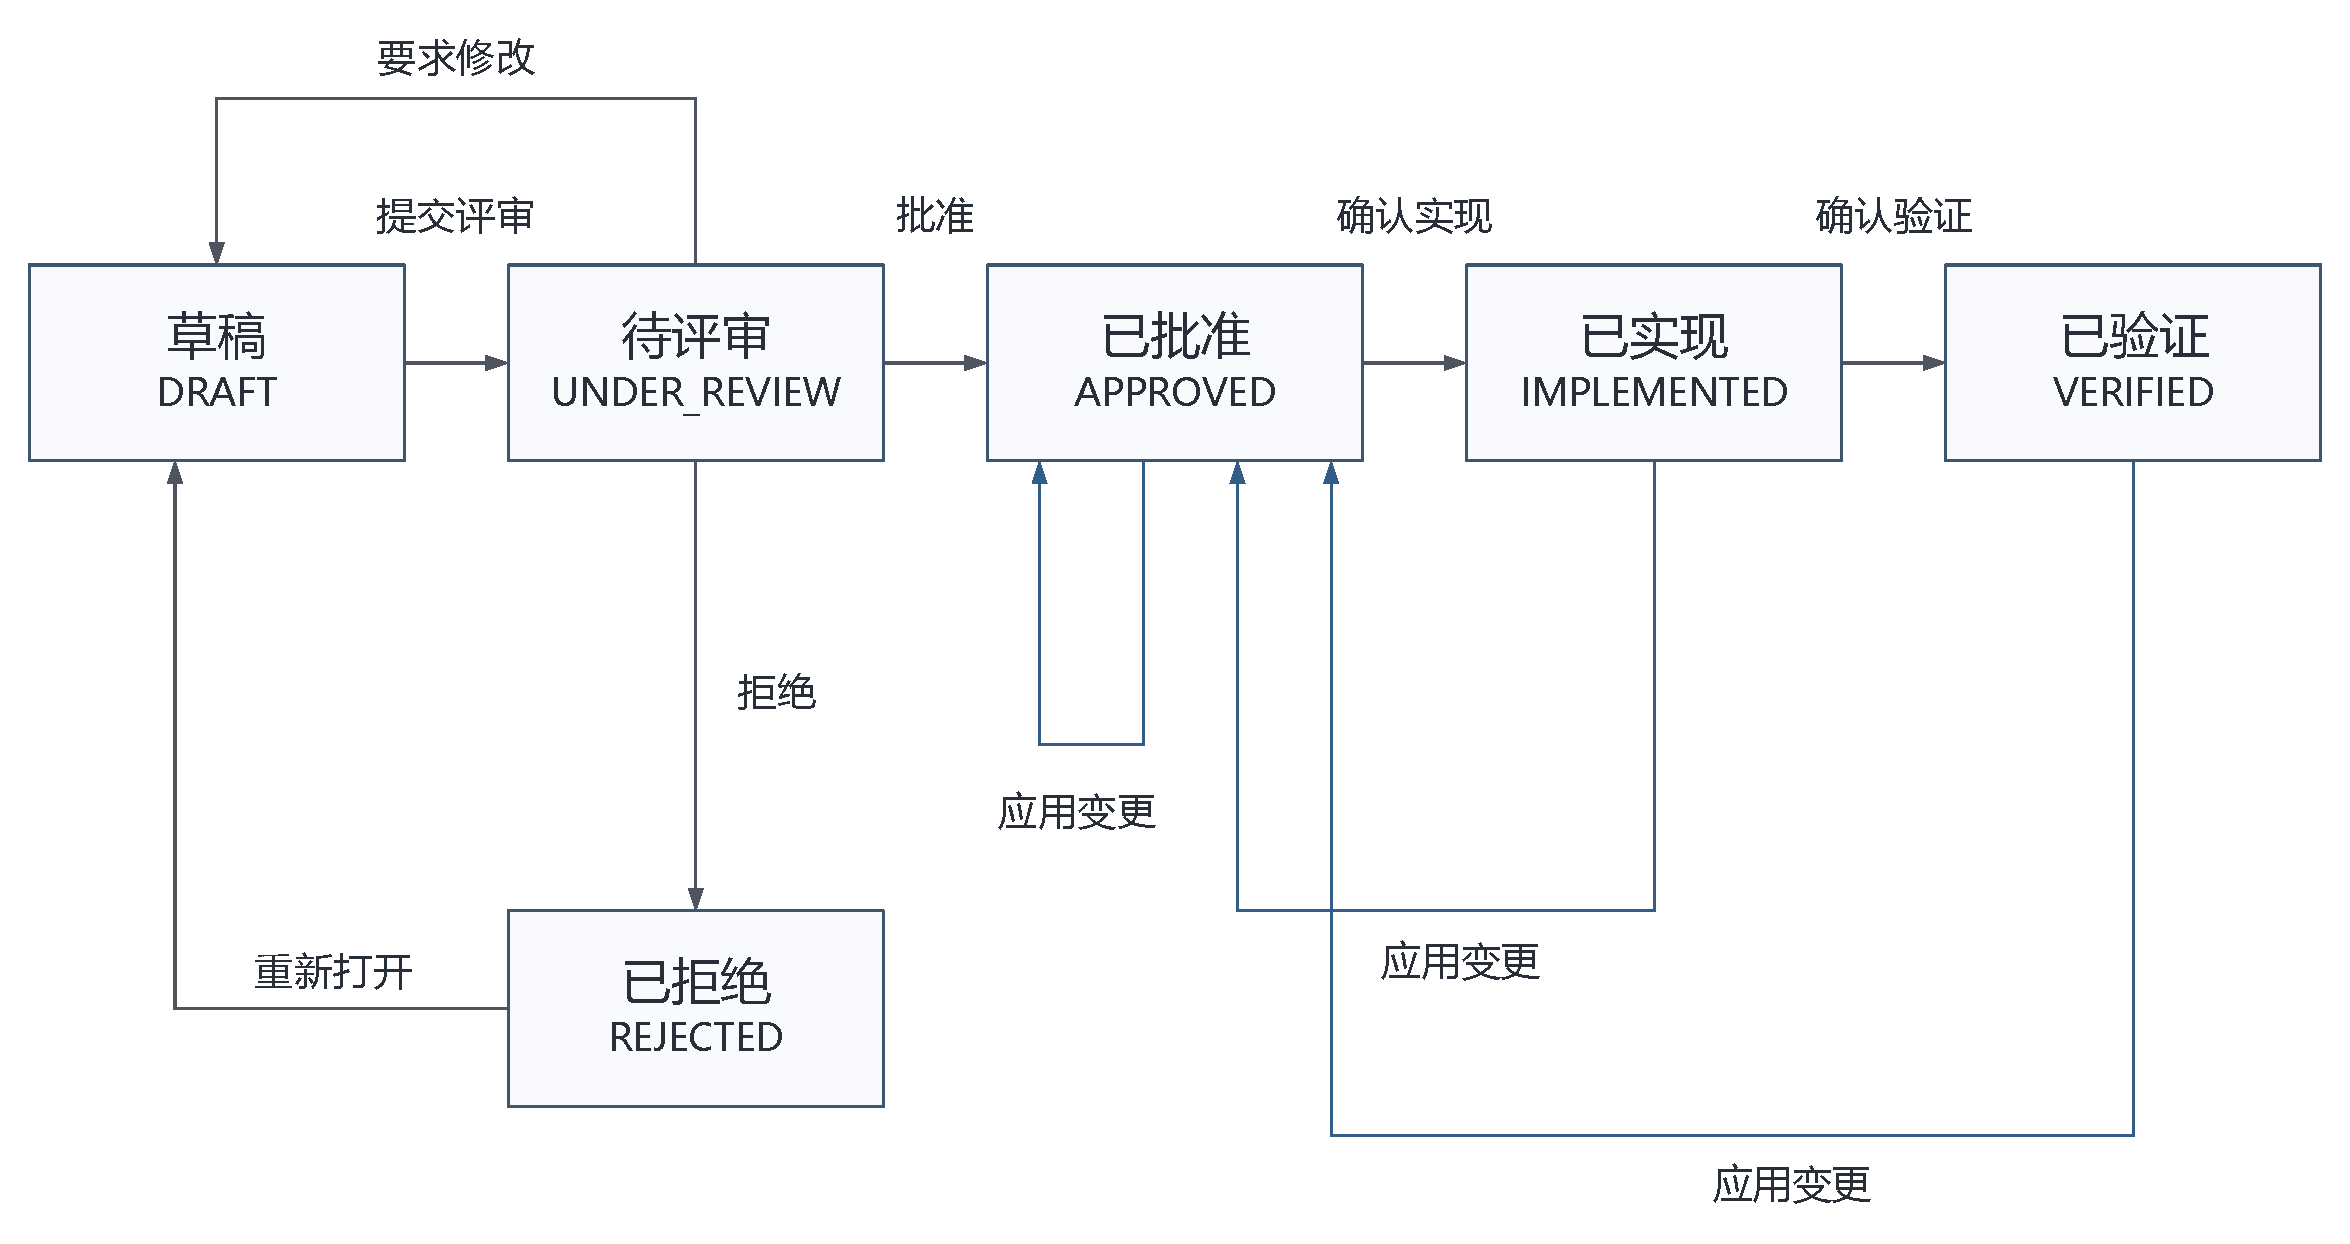
\includegraphics[width=\textwidth]{../docs/design/requirement-state.pdf}
\caption{需求状态：新正式内容需要重新确认实现和验证}\label{fig:reqstate}
\end{figure}
\begin{figure}[H]\centering
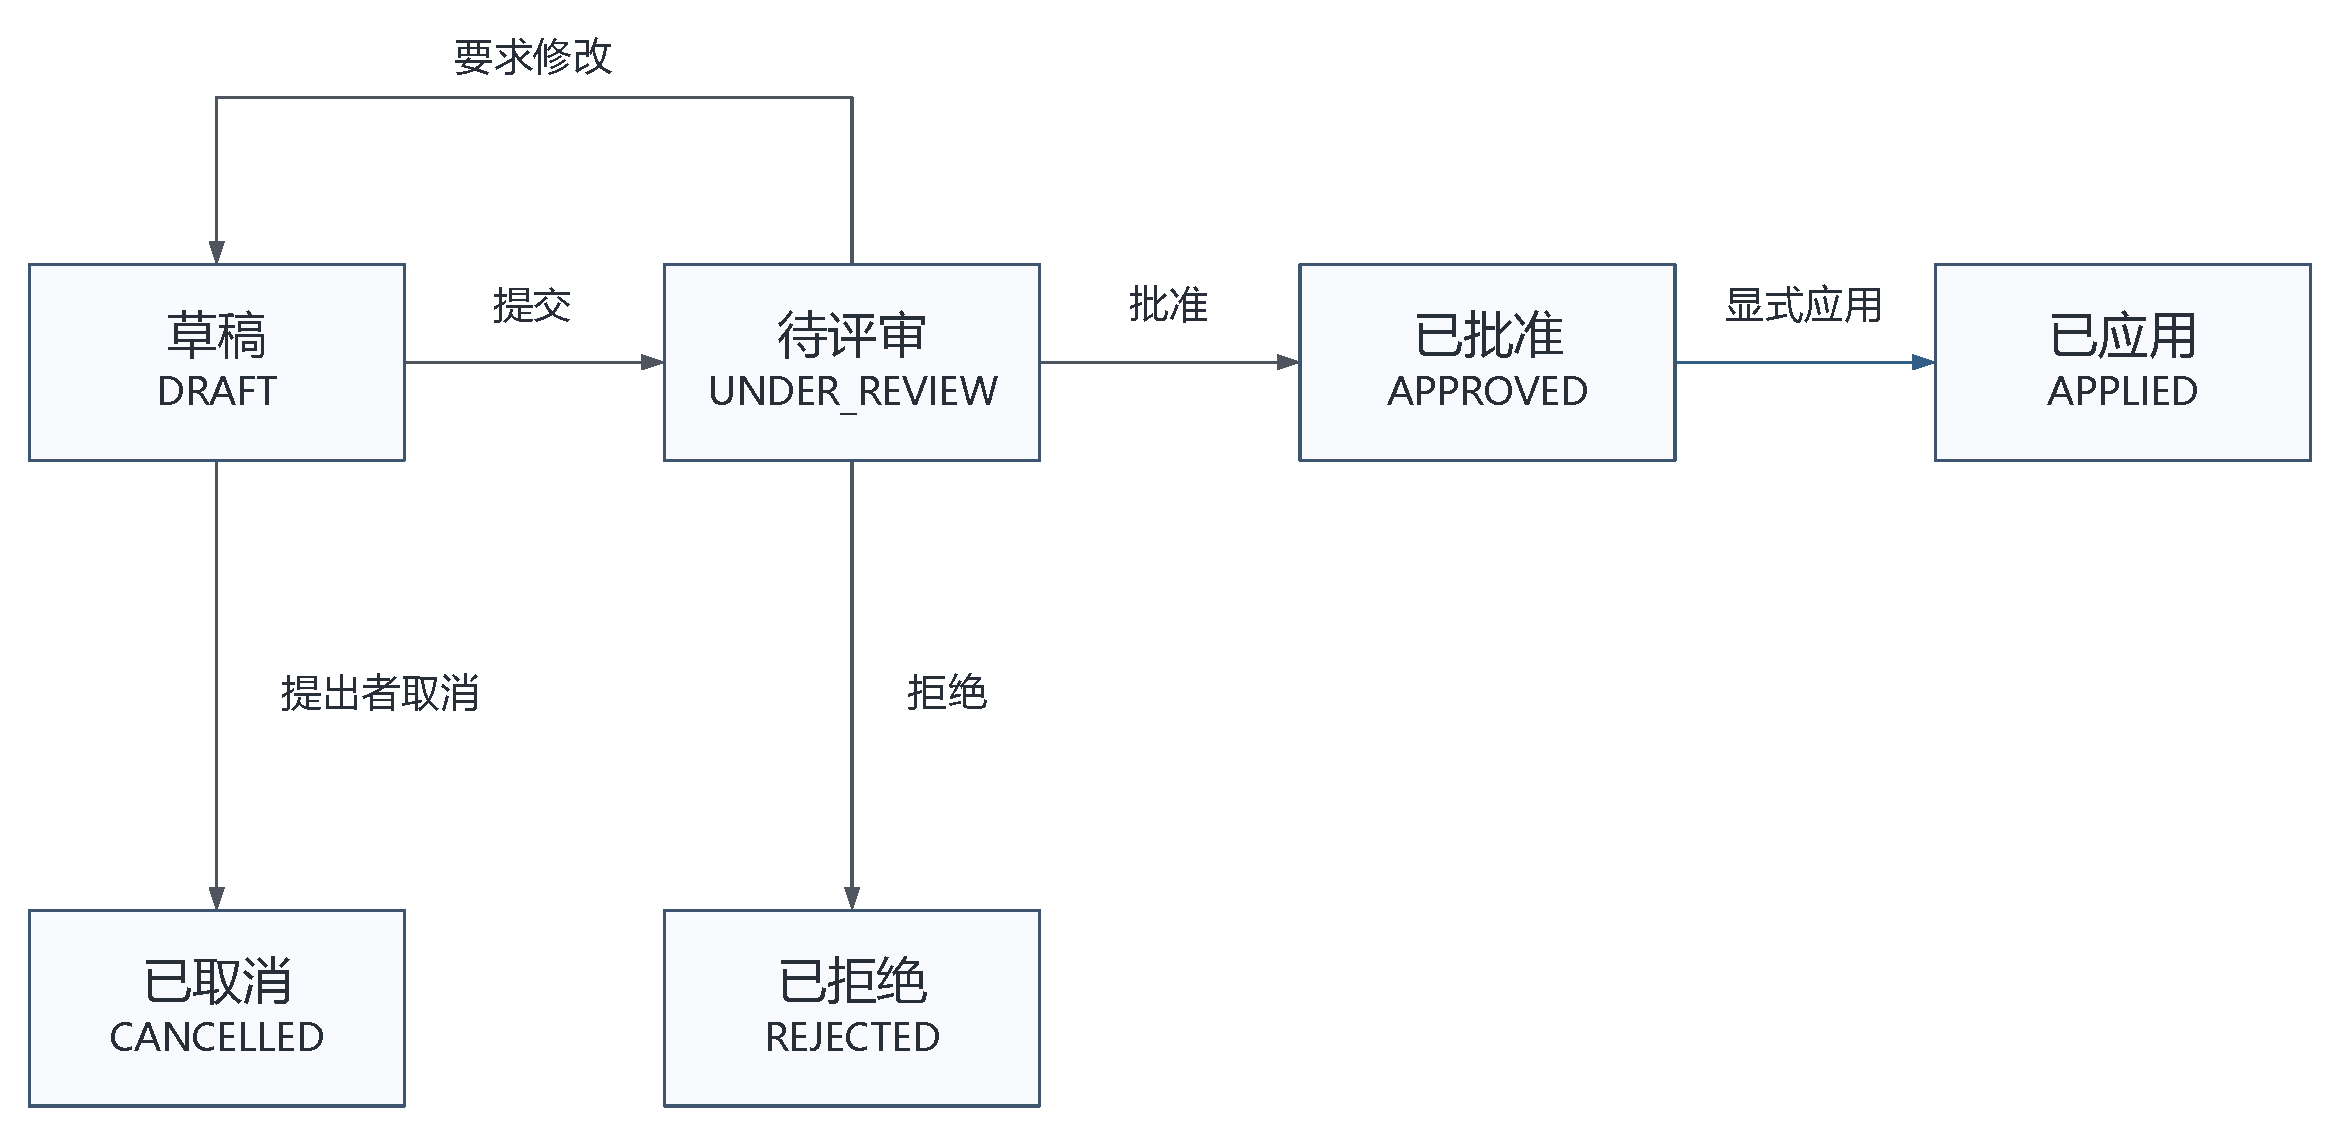
\includegraphics[width=\textwidth]{../docs/design/change-request-state.pdf}
\caption{变更状态：批准与应用分开}\label{fig:crstate}
\end{figure}

图\ref{fig:reqstate}中，首次批准创建需求正式 V1。批准、实现或验证以后应用变更，
需求统一回到已批准，不能把旧版本的实现、验证结论自动沿用到新内容。
图\ref{fig:crstate}中，变更被要求修改后回到草稿，再提交形成新轮次；拒绝、取消和
已应用是终态，不能通过直接写字段重新提交。批准变更仍不创建版本。

状态转换时，服务端还要检查权限，确认需求没有被撤销、内容完整、不是自评，并
核对评审轮次和修订号。

\subsection{系统架构选择}
一次变更应用会同时修改版本、需求、变更和审计。如果把这些模块拆成各有数据库
的服务，任何一步失败都要处理跨服务一致性。课程系统的业务范围较小，我最后采用
模块化单体，让这次操作直接使用同一个数据库事务。

Vue 3 承担页面和交互，Spring Boot 在一个进程内按用户、需求、评审、版本、变更、
关系和审计分工，MySQL 保存关系数据。模块之间有明确接口，关键写动作共同提交，
失败时统一回滚。各模块不能完全独立部署和扩容，这是当前架构保留的限制。
\begin{figure}[H]\centering
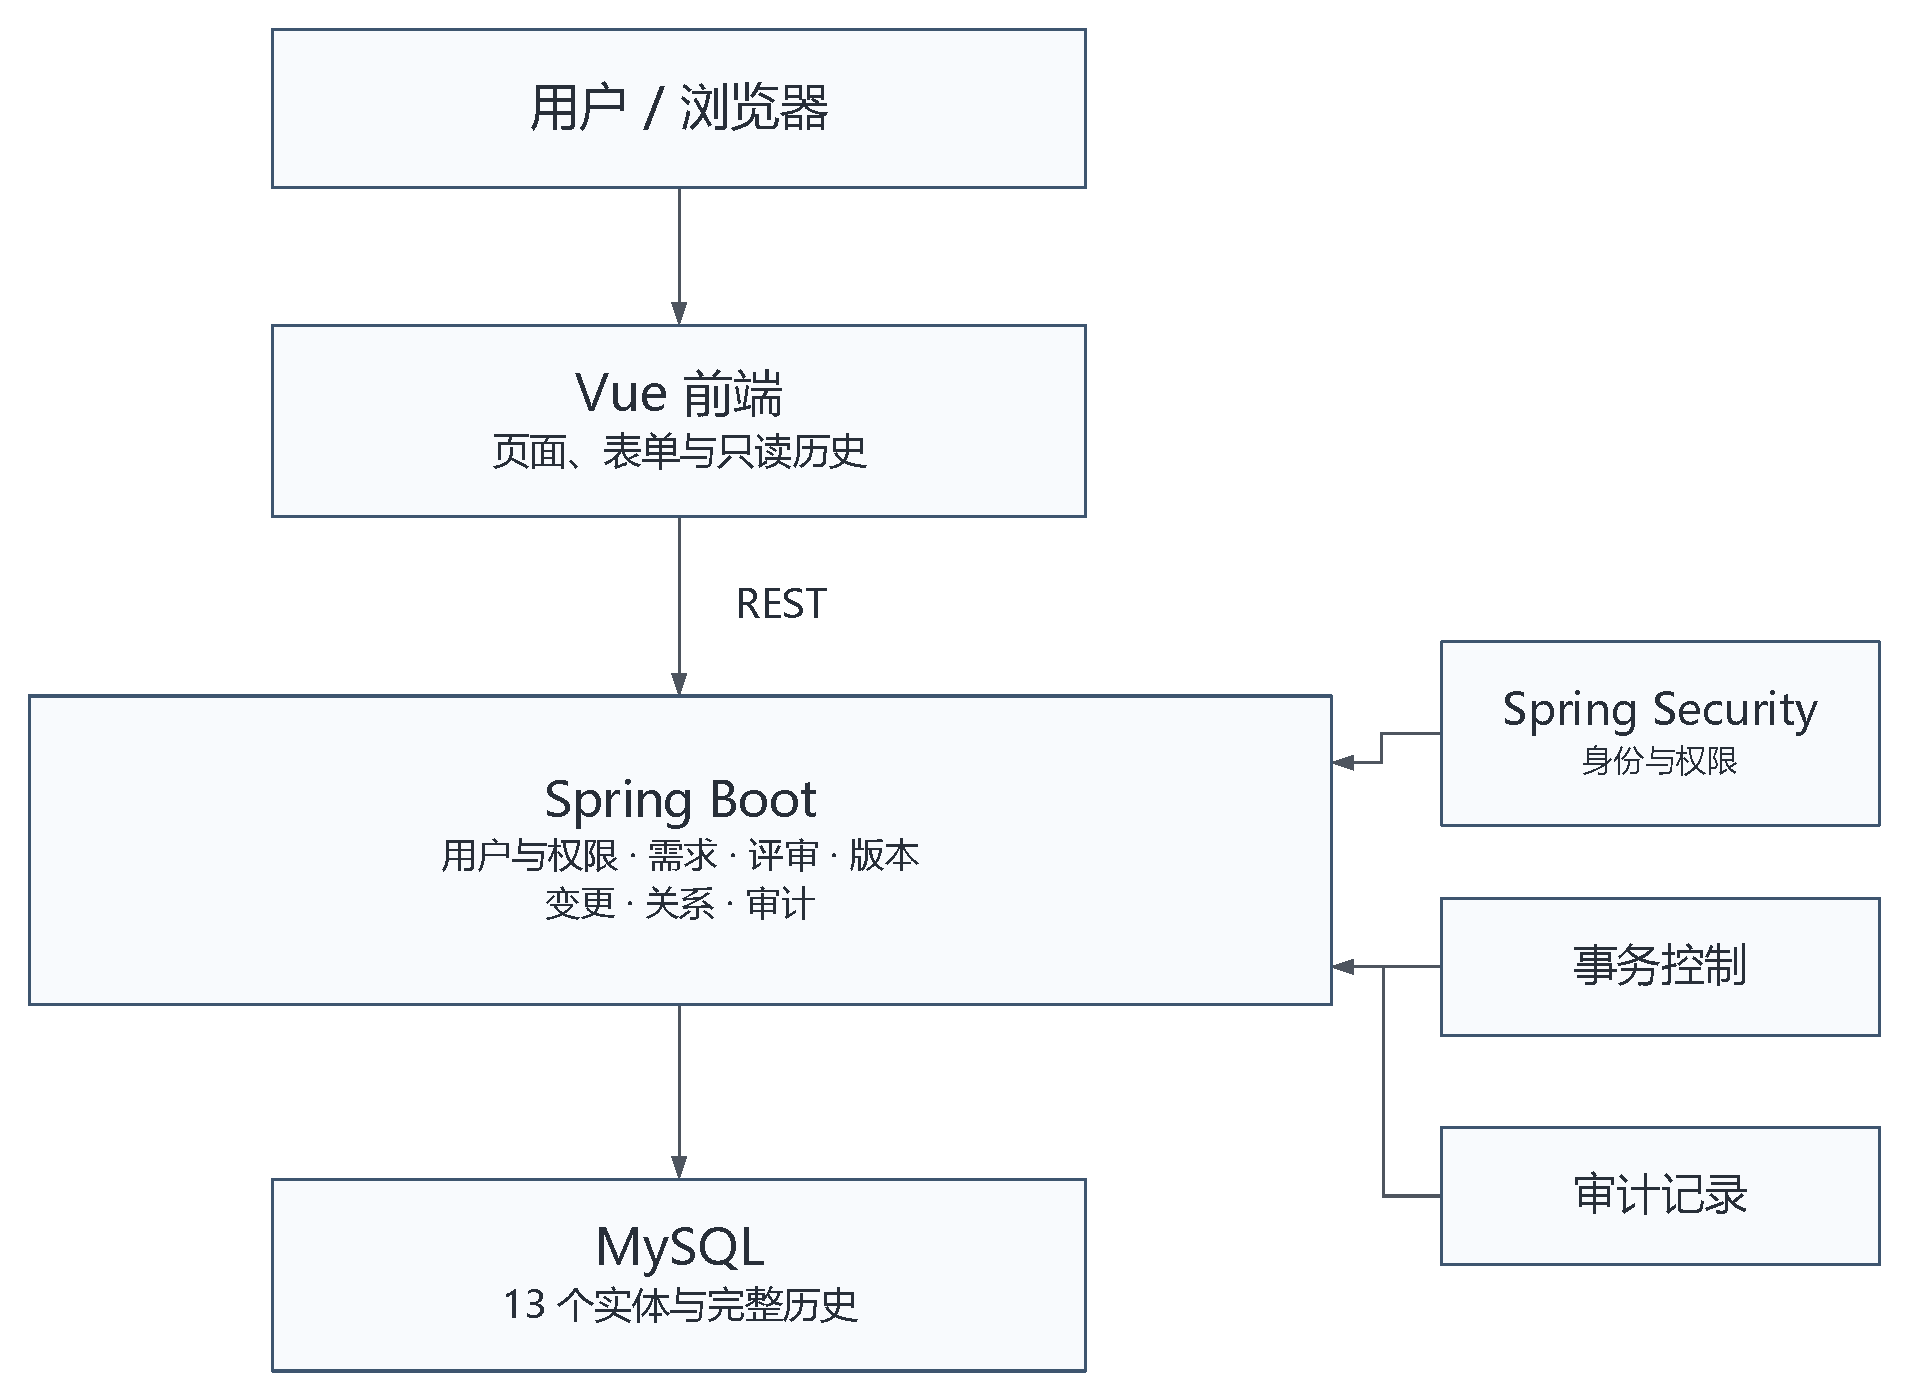
\includegraphics[width=0.94\textwidth]{../docs/design/architecture.pdf}
\caption{课程系统的前端、业务服务和数据库}\label{fig:architecture}
\end{figure}

页面接收输入，Controller 将请求转成动作参数，应用服务协调状态、权限和事务，
领域规则决定允许的变化，持久化层读写数据。数据库表不直接作为前端响应，避免
页面通过实体关联取得不应公开的字段。Spring Security 处理会话和授权入口，业务
服务继续检查创建者、提出者和对象状态等具体限制。

\subsection{版本、权限和事务如何落到实现}
\subsubsection{把字段编辑和业务动作分开}
内容编辑、负责人和标签修改、提交、决策、应用使用不同接口。客户端的请求只能
修改内容，状态和版本必须由对应的业务动作推进，否则一次编辑请求就可以把草稿
改为已批准。表\ref{tab:api}列出主要接口，完整 OpenAPI 保存在公开仓库中。
\begin{table}[H]\centering\small
\caption{主要接口及其业务边界}\label{tab:api}
\begin{tabularx}{\textwidth}{C{1.5cm}Y Y}
\toprule 方法 & 路径示意 & 含义\\\midrule
POST & \code{/requirements} & 创建草稿，标识由服务端生成。\\
PATCH & \path{/requirements/{id}/content} & 仅编辑草稿八项正式内容。\\
PATCH & \path{/requirements/{id}/metadata} & 修改管理信息，不形成版本。\\
POST & \path{/requirements/{id}/submit} & 检查并建立评审轮次、快照。\\
POST & \path{/requirement-reviews/{id}/decision} & 决策有效轮次，批准首次形成 V1。\\
POST & \path{/changes/{id}/submit} & 提交变更并复制完整申请快照。\\
POST & \path{/change-reviews/{id}/decision} & 只批准申请，不应用内容。\\
POST & \path{/changes/{id}/apply} & 检查基准并原子产生新版本。\\\bottomrule
\end{tabularx}
\end{table}

路径示意省略统一 API 前缀。操作者来自会话；角色、状态、版本号和审计时间由服务端
确定。修订号用于判断用户是否仍基于自己刚读到的对象操作。旧修订不能覆盖已经
改变的数据，冲突返回明确结果，页面重读以后再决定如何处理。

\subsubsection{一次应用的事务边界}
考虑一个反例：先插入新版本，随后更新需求失败。如果两步各自提交，版本列表里有
V2，当前指针却仍是 V1，用户会看到相互矛盾的结果。因此应用变更的完整动作包括：
锁定需求与变更；复核批准状态和基准；追加下一版本；复制批准内容并更新当前指针；
把需求置为已批准；把变更置为已应用；写入成功审计。这些步骤在同一个事务里提交，
任何一步失败都不会留下部分成功的结果。

数据库负责真实外键、唯一键和活动占用约束，业务服务负责权限、自评、合法转换、
连续版本号和依赖环等语义。并发创建两个活动变更时，不能只靠“先查询再插入”；
串行化与数据库约束共同避免两个请求都认为没有活动变更。重复审批和应用也需要
在锁定后再次检查，不能依赖按钮只被点一次。

成功审计随业务修改一起提交。失败审计在主事务结束后独立记录，避免失败记录随
主事务回滚而被删除。失败观察还要保留原异常的含义，并且把已经提交的操作和未
提交的失败区分开，不能让失败记录写错事务结果。

\subsection{系统界面与主要功能}
界面应帮助使用者区分当前内容、正式版本和历史提交。需求工作区提供筛选、分页
和详情，详情用概览、版本、评审、关系、变更、评论和历史页签组织内容。状态和
当前版本放在管理信息区，描述、理由与验收标准放在正式内容区。

图\ref{fig:detail}与图\ref{fig:change}来自独立的展示数据库，分别展示需求内容，以及
变更基准、建议内容和应用结果。截图里的用户和需求都是演示数据，实验结论另按原
测试记录统计。“邮件通知”与“需求导出”这类标题只是需求文本，没有对应的产品功能。
这两张图取自经过展示调整的版本：布局、CSS、显示组件和文案有过改动，业务接口、
路由、权限和动作未变，本次只裁去了截图外围的留白。
\begin{figure}[H]\centering
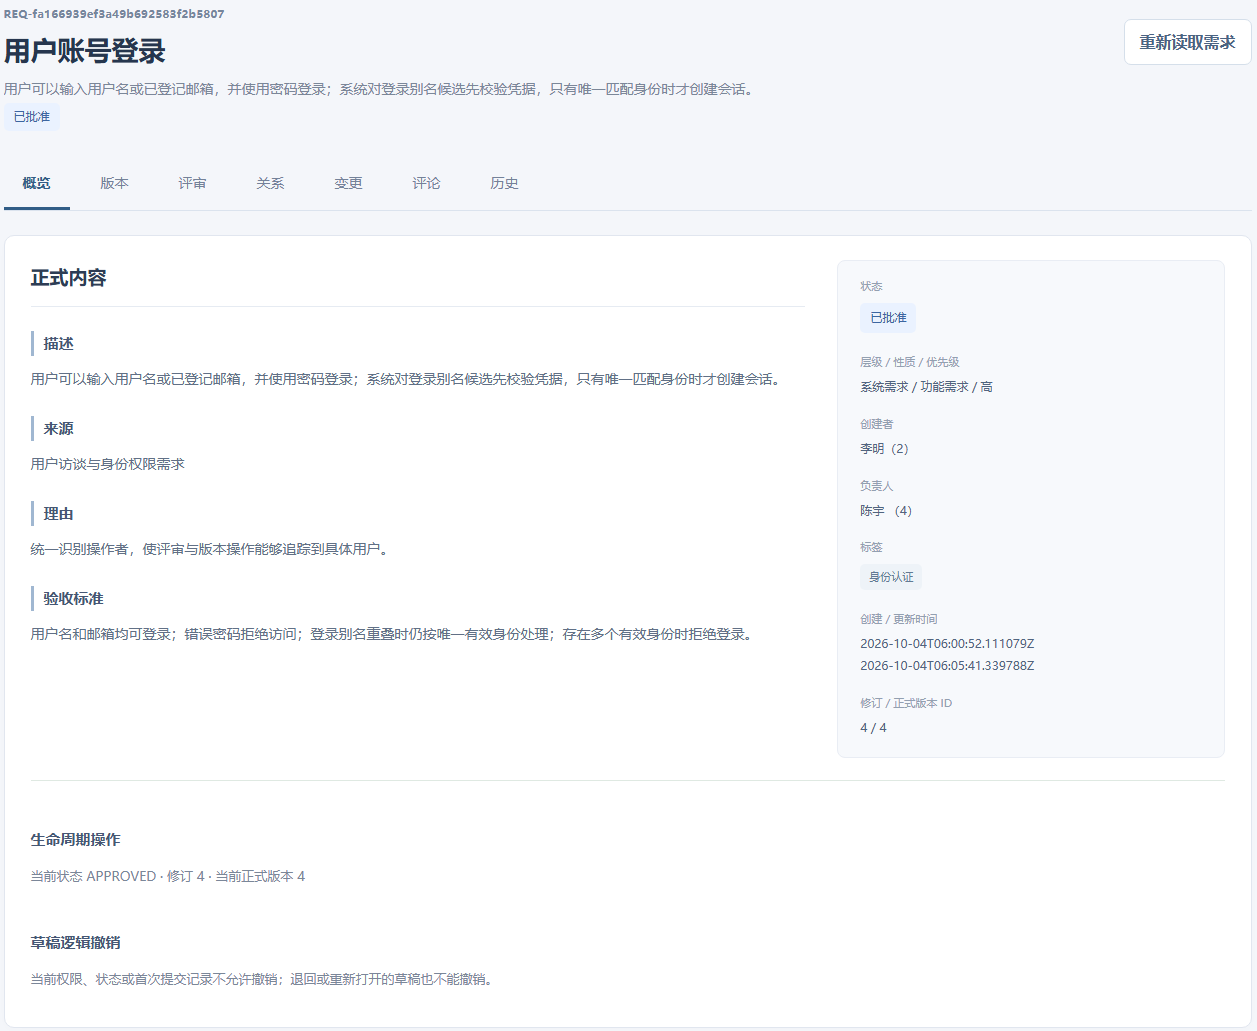
\includegraphics[width=\textwidth]{../docs/screenshots/requirement-detail.png}
\caption{需求详情：正式内容与管理信息分开呈现}\label{fig:detail}
\end{figure}
\begin{figure}[H]\centering
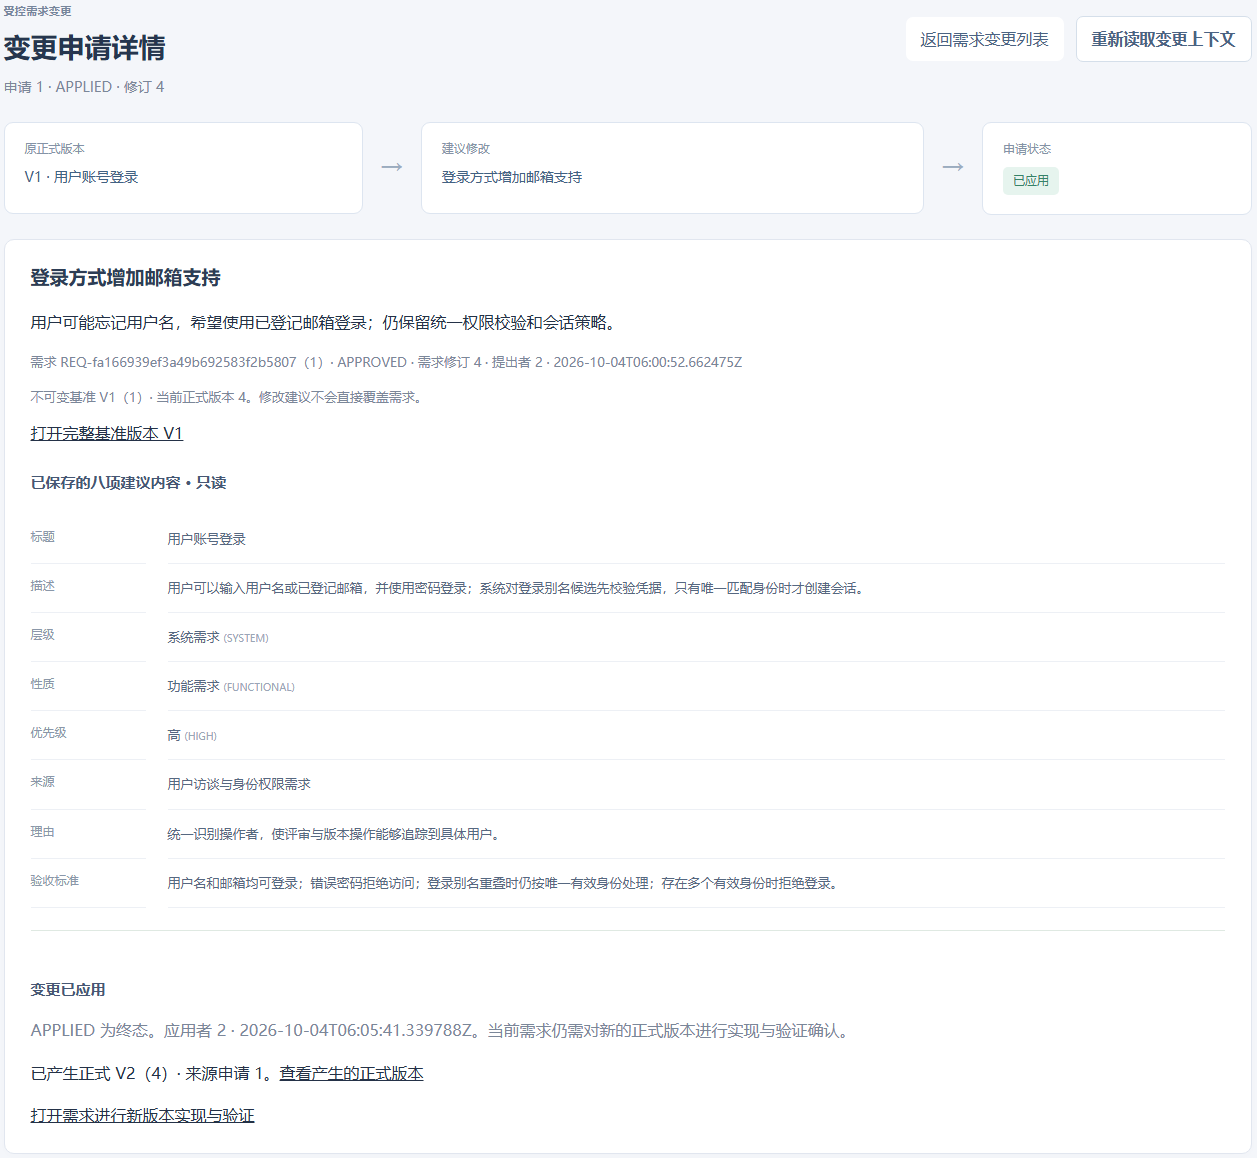
\includegraphics[width=\textwidth]{../docs/screenshots/change-request.png}
\caption{变更申请：从基准版本到建议内容，再到批准和应用}\label{fig:change}
\end{figure}

数据模型、状态规则和接口边界至此都已确定。接下来要说明的是，同一份设计交给
多个 AI 角色实现会得到什么结果。
\chapterbreak
\section{多智能体辅助实现}
\subsection{单一 AI 工作方式的问题}
同一个 AI 如果同时解释需求、写代码和编写测试预期，一次错误理解可能同时进入
实现和测试。两边相互吻合，测试就可能通过，而实际业务规则仍被误解。

我把预期交给需求和测试角色，前后端角色依据已确定设计实现，再由审查角色检查
代码。角色之间需要交接，也可能共享错误假设，因此运行结果仍要落实到具体请求、
页面操作和数据库后果。原始记录保留下来，便于核对问题是否真的发生。

\subsection{我的智能体分工}
实际协作包含需求追踪、架构、前后端实现、测试、审查和受约束重构几个逻辑角色。
表\ref{tab:agents}列出各自的判断依据；图\ref{fig:agents}只表示实际工作顺序，
内部编号和过程文件不作展开。
\begin{table}[H]\centering\small
\caption{协作角色及相互检查的关系}\label{tab:agents}
\begin{tabularx}{\textwidth}{C{2.7cm}Y}
\toprule 角色 & 职责与判断依据\\\midrule
需求追踪 & 把需求、规则、用例和检查场景对应起来，发现遗漏和歧义。\\
架构 & 说明模块接口、状态守卫、事务和数据边界。\\
后端、前端实现 & 按共同设计实现，不能自改需求预期。\\
测试 & 用既定场景运行真实 HTTP、浏览器和数据库，保留失败。\\
代码审查 & 只读分析代码路径、根因及范围，区分观察与推测。\\
重构 & 依据被接受问题和明确约束修改，再接受同一场景检查。\\\bottomrule
\end{tabularx}
\end{table}
\begin{figure}[H]\centering
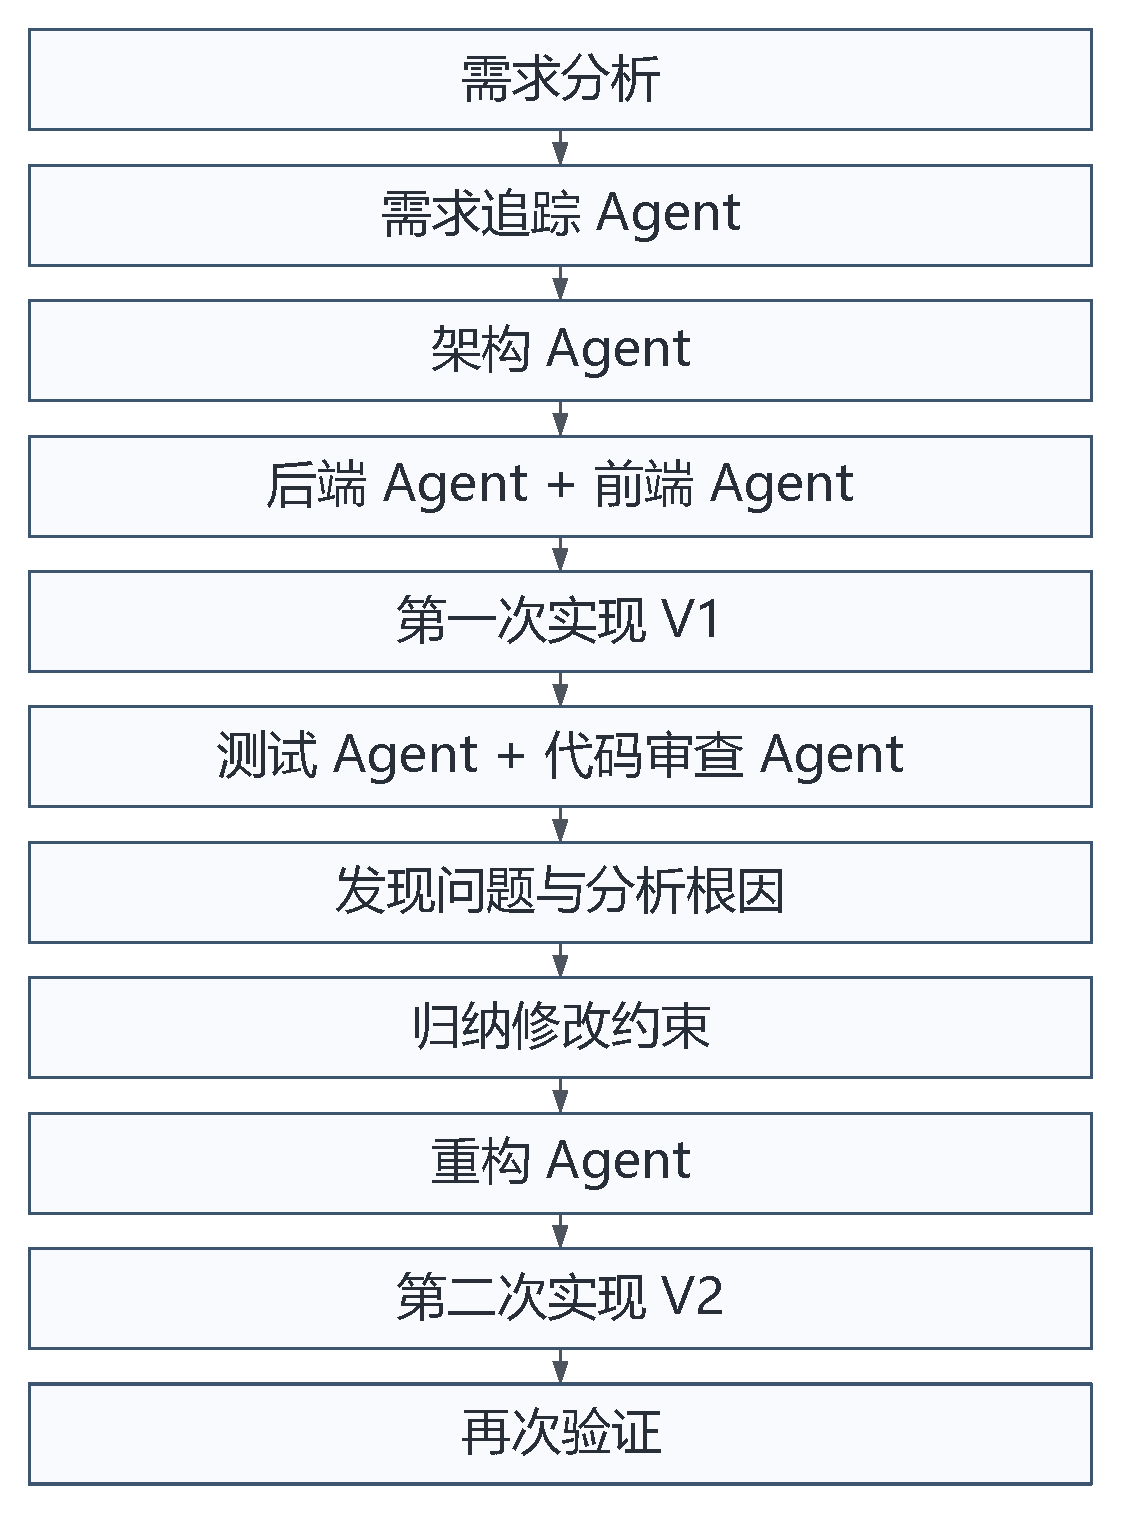
\includegraphics[height=0.36\textheight]{../docs/design/multi-agent-workflow.pdf}
\caption{从共同设计到独立检查，再到受约束的改进}\label{fig:agents}
\end{figure}

\subsection{第一版是怎样产生的}
实现开始以前，几个角色要先对评审快照、正式版本和变更应用形成一致理解。如果
后端把批准变更理解为马上生成版本，而前端把它理解为等待显式应用，两边都可能
各自编译成功，却无法连成同一业务过程。因此需求和架构角色先确定输入输出、
动作前提和后果，前后端再按这些约定分工。

实现沿着用户权限、需求维护、评审与版本、变更和追踪这几条线，逐步形成可运行
流程。开发检查帮助及时发现类型、接口和模块依赖问题；它们属于生成阶段的反馈，
不能与后续独立实验混为同一批计数。第一版固定下来以后，才用代表性场景观察它
的实际行为。

\subsection{如何避免 AI 自我验证}
业务预期和第一次实现分开保存，测试阶段固定第一版代码，实现角色不边运行边修改。
测试报告记录实际请求、页面旅程和数据库后果，代码审查再把运行观察对应到具体
分支。静态风险和运行失败分别记录，失败时也检查环境和脚本定位是否正确。

问题核实以后，重构只处理已确认的根因。修改完成以后仍用同一批场景和预期复查，
失败场景保留在结果中，通过条件没有放宽。我核对问题记录、实际修改和复查结果，
确认修改守住了已经确定的业务规则。

下一节说明这次检查选定了哪些场景、结果如何，以及发现的四个问题。

\chapterbreak
\section{第一版代码的实际检查}
\subsection{测试选择}
完整设计列出 103 项检查，本次实际执行了其中 32 个代表性原设计场景。选择这些
场景时，我优先覆盖身份和权限、需求提交和决策、正式版本、变更应用，其次覆盖
事务、并发和两条完整的浏览器旅程。这几处是设计中最关键的部分：权限决定谁能
推进流程，正式版本从提交和决策产生，变更应用一次要同时写版本、需求和变更
几张表。协议、认证边界和查询计数的补充检查单独统计。

剩下 71 项仍标为未运行，部分代表场景里也有没覆盖到的变体。开发阶段的单元检查与
独立实验分开统计，两版都沿用这 32 个场景的计数口径。

检查不只看 HTTP 是否成功。例如应用变更以后，需要同时确认当前指针、正式版本
八项内容、申请状态和审计；自我评审即使按钮不存在，也要通过直接请求验证后端拒绝。
事务故障场景则观察失败以后是否完整回滚，避免只根据异常响应推断数据库状态。

\subsection{第一版结果}
应用 V1 的 32 个代表场景中，31 项通过，1 项失败，阻塞为零。两条浏览器旅程和
已执行的状态、权限及事务反例未显示业务结构被破坏，但这不能替代未运行范围。
表\ref{tab:v1results}把这几类数字分开列出：代表场景的计数、没有运行的部分、
那次失败的结果，以及补充检查能说明和不能说明的边界。
\begin{table}[H]\centering\small
\caption{第一版检查的口径}\label{tab:v1results}
\begin{tabularx}{\textwidth}{C{4.5cm}Y}
\toprule 内容 & 实际结果与适用范围\\\midrule
原设计代表场景 & 32 项：31 PASS、1 FAIL、0 BLOCKED。\\
其余原设计场景 & 71 项 NOT\_RUN，部分未覆盖变体另行注明。\\
运行失败 & 不同密码的交叉登录别名导致两个合法账号均被拒绝。\\
独立补充与审查 & 协议分类、分页查询次数、重复失败观察模板及事务可读性。\\
本次未覆盖 & 生产负载表现、全面安全性和所有并发组合都没有实测。\\\bottomrule
\end{tabularx}
\end{table}

\subsection{四个有代表性的问题}
登录别名是这 32 个场景中唯一失败的一项。另外三个问题来自场景之外的补充检查和
代码审查，单独计数，不计入这 32 项。四个问题都留有代码位置或复现步骤。
\subsubsection{登录别名：字段唯一不等于入口唯一}
我在登录检查中使用一个合法组合：用户甲的邮箱等于用户乙的用户名，两人的密码
不同。用户名列和邮箱列各自都不重复，但共享“用户名或邮箱”入口以后，可以同时
查到两个不同账号。第一版在校验密码之前就假设只能找到一个账号，因此两次正确
密码登录都被拒绝。

第一版从两个数据列各自唯一出发，认为登录入口也只能匹配一个身份。这个账号组合
符合原数据规则，修改时仍需支持它，不能直接拒绝账号或规定用户名优先。第二版
先取得不同身份候选，再通过密码匹配确定唯一身份，BCrypt 算法和列唯一规则保持
原样。

\subsubsection{协议异常：把错误请求误记成服务器故障}
对已存在路径使用不支持的方法，或向需要 JSON 的接口发送不支持的媒体类型，第一版
都返回 500。补充 HTTP 检查使用有效认证和 CSRF 令牌，检查前后的会话查询均成功，
排除了会话失效被误判为协议问题的可能。

全局错误处理已经接管框架异常，但客户端异常白名单遗漏了这两类情况，它们落入
默认的内部故障分支。这里的问题是分类边界不完整，不能通过把所有异常改成 400
解决，否则真正的服务器故障又会被隐藏。

\subsubsection{分页查询：单条详情的做法不适合整页}
第一版把读取单条需求的组装函数用在分页结果的每一行。这个函数内部还要查一次
标签，把它逐行复用，标签查询也就逐行执行，因此 1 行和 20 行结果页分别产生
1 次和 20 次标签 SELECT。实际查询计数支持了代码审查提出的 N+1 问题，返回内容
本身仍然正确。

分页场景需要先从整页收集需求标识，再批量读取标签。这次记录的是标签 SELECT
次数，没有测量响应时延或生产吞吐。

\subsubsection{失败观察和关键事务：复制模板增加修改风险}
六个写操作业务入口各自复制了一份失败观察模板，其中包含失败目标定位、权限拒绝
分类、独立审计和异常重抛；变更应用的多个重要步骤又写在很长的单行代码中。
代码能够执行，但审阅一个步骤是否仍在原事务内，以及未来修改是否漏改另一份模板，
都更困难。

这是维护性和职责组织上的问题。现有证据只显示模板重复和可读性差，没有显示第一
版部分提交过，或者写入过假的成功审计。修改需要集中稳定的技术规则，使关键
步骤可读，同时保持原有事务边界和业务守卫。

\subsection{这些问题为什么会出现}
登录代码依赖了错误的唯一性假设，错误处理遗漏了两类客户端协议异常，分页逐行
复用了带 SQL 的组装函数，失败观察的模板又在六个业务入口各写了一份。后来检查
一次变更应用，需要跨多个位置核对同一套规则。

各实现角色按模块完成任务，容易先处理单个接口或单条数据。登录入口同时使用
用户名和邮箱、分页一次处理多条需求、业务写入还带有审计，这些关系要把模块放在
一起检查。我在测试和审查中把具体观察对应到这些假设，再确定每处修改的范围。

\chapterbreak
\section{第二版修改与验证}
\subsection{根据第一版问题确定修改原则}
第一版的问题核实以后，我把每处必须改变的行为和需要保持的规则分别写下来，见
表\ref{tab:constraints}。登录修复要支持原来合法的账号组合，协议错误要沿用已有
响应合约，分页优化要保持返回内容，维护性调整要保留事务和失败审计边界。设置
这两列以后，重构时每一步都有具体条件可核对。

\begin{table}[H]\centering\small
\caption{由实际根因形成的四条修改约束}\label{tab:constraints}
\begin{tabularx}{\textwidth}{C{0.9cm}Y Y}
\toprule 编号 & 必须改变 & 必须保持\\\midrule
1 & 对每个不同用户名/邮箱候选校验，只在恰好一个密码匹配时选择身份。 & 原账号取值域、列唯一性、禁用检查及 401 身份拒绝；不泄露候选与哈希。\\
2 & 显式分类不支持方法和媒体类型，映射为已有 400 输入错误。 & 真正内部错误仍为 500，原 401、403、409 和脱敏响应不变。\\
3 & 非空需求页一次批量读取全部标签，按原顺序组装。 & 分页、总数、标签顺序、DTO 内容和单条详情语义不变。\\
4 & 六个业务入口共用窄失败观察契约，变更事务步骤易读。 & 独立失败审计、原异常、已提交清理特例和应用单事务不变。\\\bottomrule
\end{tabularx}
\end{table}

这轮修改保持原数据模型和状态机，第二版形成后仍按原场景和预期检查。

\subsection{第二版的主要修改}
认证读取至多两个不同身份候选，固定进行两个 BCrypt 比较，不足的候选用占位哈希
补齐。恰好一个匹配后，再检查该身份启用状态；零个或多个匹配仍拒绝。这样修复了
不同密码的交叉别名情形，而没有用角色或记录顺序任意选择用户。

错误处理加入两类已复现协议异常的明确映射，采用系统已有的
\code{INVALID_INPUT/400}。通用 HTTP 处理常用 405、415，这次修改沿用原系统的
输入错误合约，没有新增这两种业务响应。

分页先从本页收集需求标识，一次读取这些需求的全部标签，分组之后再按原顺序组装，
单条详情的行为保持原样。失败观察则集中到审计模块的窄契约，由调用方提供
可信操作者和目标上下文；它不包围业务事务，也不接管各模块的角色、状态和自评
守卫。应用变更拆成可读步骤，仍然一次提交。

\subsection{两版结果比较}
两版使用相同的 32 个原设计场景、预期和运行脚本。应用 V1 为 31 项通过、1 项失败，
应用 V2 为 32 项通过、零失败，原来的登录失败场景在第二版通过。运行结果、补充
观察和开发检查分别列在表\ref{tab:comparison}中。
\begin{table}[H]\centering\small
\caption{相同口径下的两版比较}\label{tab:comparison}
\begin{tabularx}{\textwidth}{Y C{3.0cm}C{3.0cm}}
\toprule 项目 & 应用 V1 & 应用 V2\\\midrule
原代表场景通过/失败 & 31 / 1 & 32 / 0\\
原设计未运行 & 71 & 71\\
不同密码交叉别名登录 & 两个正确身份被拒绝 & 各自密码识别各自身份\\
两类补充协议错误 & 500 内部错误 & 400 既有输入错误\\
1 行/20 行页标签 SELECT & 1 / 20 & 1 / 1\\
失败观察模板 & 六处重复 & 统一窄契约\\
开发阶段后端检查 & 45 项 & 72 项（含 27 项新增定向检查）\\
开发阶段前端检查 & 152 项 & 152 项\\\bottomrule
\end{tabularx}
\end{table}

四处事务故障和已执行的重复、并发及权限场景继续保持预期结果。查询次数和认证
边界检查单独统计。此前进行展示布局调整时重新运行了原来的两条浏览器旅程，
两条流程保持原结果。

如果两个不同账号共享同一别名，输入密码又同时匹配两者，系统仍返回 401。现有
输入不足以区分身份，所以不会按启用状态、角色或用户名优先级任选一个账号。
解决这一情况需要新的身份区分规则，本轮保留原账号语义。

\chapterbreak
\section{我的结论}
实现交给 Codex 的 subagent，按固定顺序推进。需求追踪 Agent 核对需求、规则、用例
和检查场景能否对应；架构 Agent 确定模块接口、状态守卫和事务边界；后端 Agent
与前端 Agent 依据同一份设计分别实现。第一版出来以后我把代码固定住，由测试
Agent 和代码审查 Agent 独立检查，测试预期在实现之前就已写好。问题核实以后，
我把每处根因写成约束，交给重构 Agent 做第二版，再用同一批场景复查。生成代码
那一段，我主要提要求和审阅结果。

四个问题里，登录别名最让我意外。我以为用户名列和邮箱列各自唯一，登录入口也就
唯一，所以第一版在校验密码之前就假定只能查到一个账号。用一对合法数据登录时，
甲的邮箱恰好等于乙的用户名，两人密码不同，两次正确的密码却都被拒绝。我把
唯一性当成了理所当然的前提，而它只约束了单列，没有约束“用户名或邮箱”这个
合并后的入口。

从那以后，我审阅生成代码时除了看它有没有按我说的做，还要看它默认了什么。分页、
协议异常和失败观察模板都来自没有写出来的假设。第二版按约束修改后用原场景复查，
同别名、同有效密码对应两个身份的情况仍然被拒绝，继续改代码并不能解决。

\begingroup\small\setstretch{1.1}
\begin{thebibliography}{9}
\bibitem{textbook}Jeffrey L. Whitten, Lonnie D. Bentley.\newblock
\textbf{系统分析与设计方法}，第 7 版.\newblock 需求分析、数据建模与数据库设计相关章节。
\bibitem{doors-attributes}IBM.\newblock
\emph{Creating attributes for requirement artifacts, DOORS Next 7.1.0}.\newblock
\url{https://www.ibm.com/docs/en/engineering-lifecycle-management-suite/doors-next/7.1.0?topic=projects-creating-attributes-requirement-artifacts}.
\bibitem{doors-links}IBM.\newblock
\emph{Links between artifacts, DOORS Next 7.1.0}.\newblock
\url{https://www.ibm.com/docs/en/engineering-lifecycle-management-suite/doors-next/7.1.0?topic=artifacts-links-between}.
\end{thebibliography}\endgroup
\end{document}
